% Section: Experiments
\section{Experiments} \label{sec:experiment}


%% First
\subsection{First Experiment}
Our first experiment is conducted on a one-dimensional data as shown in Figure~\ref{fig:data1}. In this experiment, we have a 543-point training set ranging from $x = -32$ to $x = 14$, and we want to predict some 67-point test set ranging from $x = 14$ to $x = 21$.

\begin{figure}[htp]
\begin{minipage}[htp]{1\linewidth}
	\centering
  	\subfloat{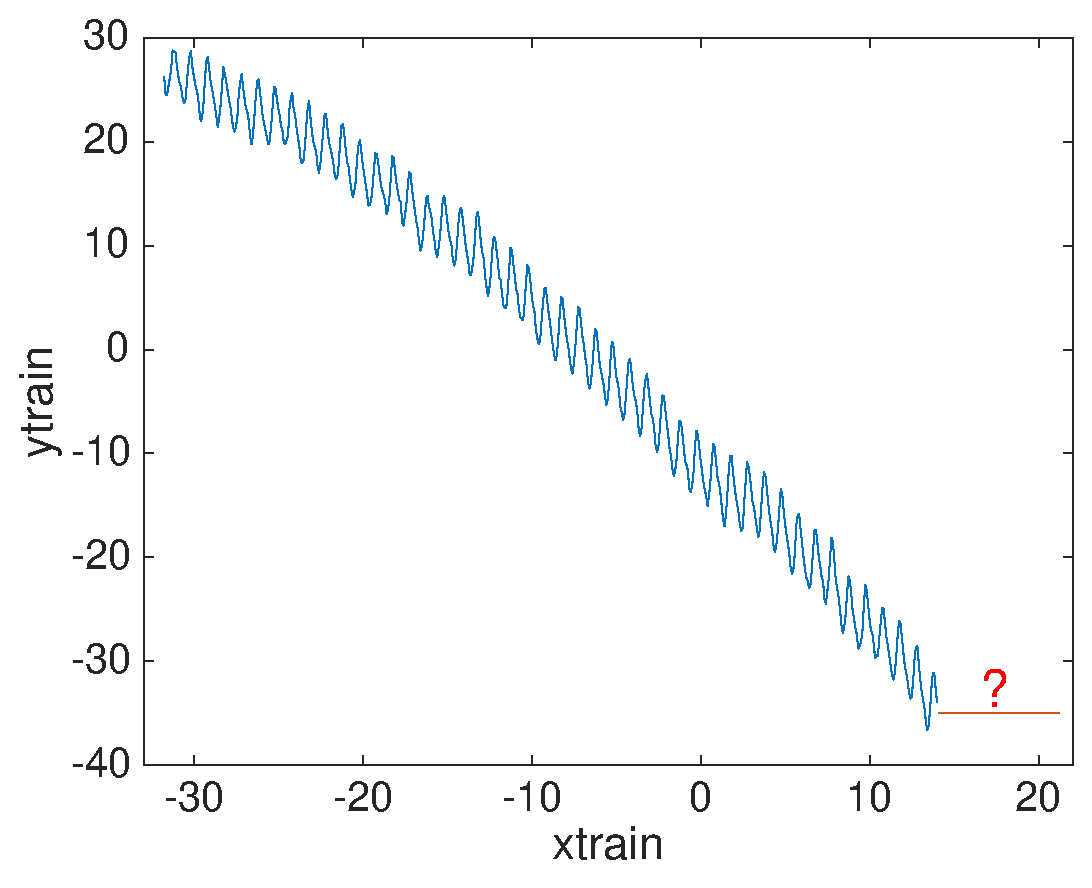
\includegraphics[width=0.7\textwidth]{figure/data1.eps}}
% \vspace{-0.1in}
\caption{A one-dimensional dataset}
\label{fig:data1} % FIG1
\end{minipage}
\vspace{-0.05in}
\end{figure}

To better do this work, we use the Auto Construction Kernel method described in Section~\ref{sec:autokernel}.
By doing a lengthy greedy kernel construction procedure, we derive a compositional kernel:
\begin{equation}
LIN \times SE + SE \times ( PER + RQ )
\end{equation}
And by using the Guassian Likelihood function and the exact posterior probability.
We predict the results as in Figure~\ref{fig:predict1}

\begin{figure}[htp]
\begin{minipage}[htp]{1\linewidth}
	\centering
  	\subfloat{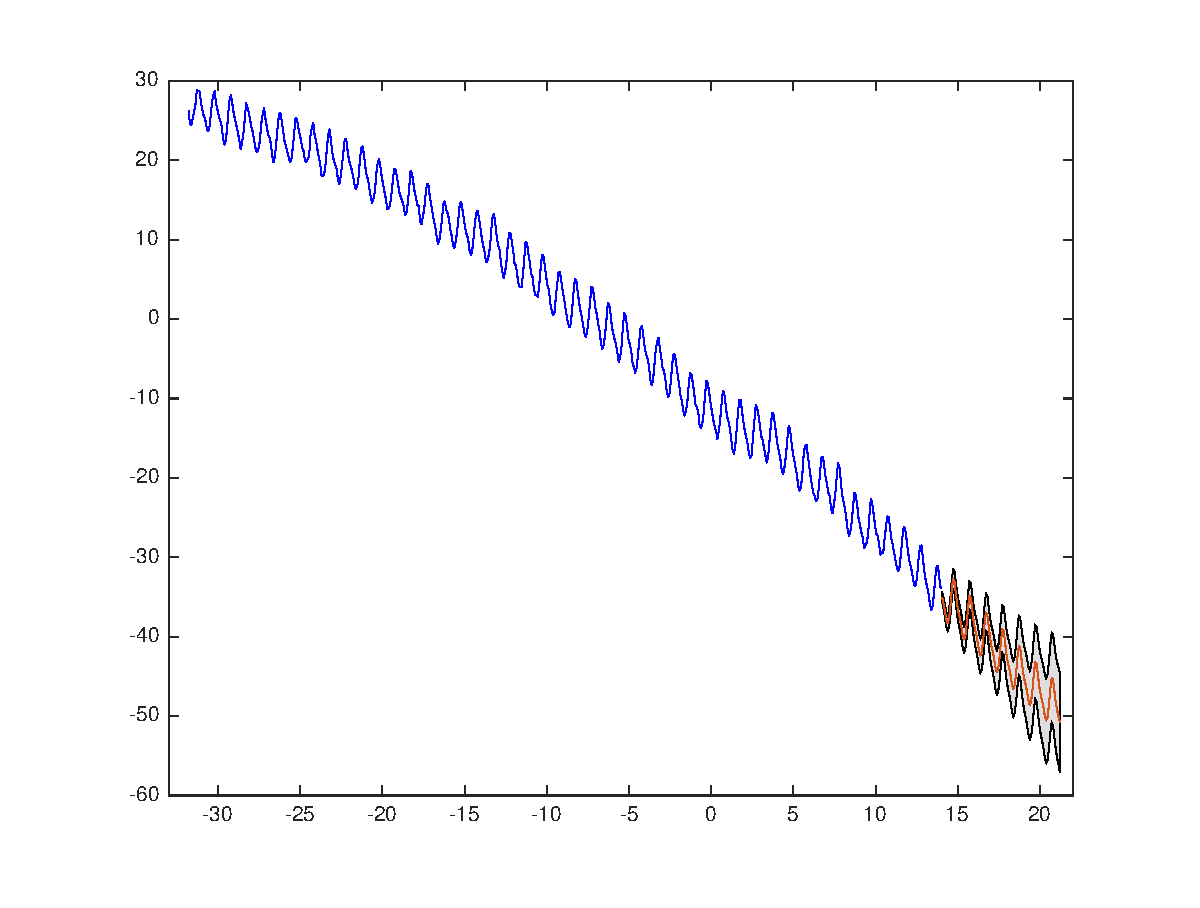
\includegraphics[width=0.7\textwidth]{figure/predict1.eps}}
% \vspace{-0.1in}
\caption{Prediction of the 1st dataset}
\label{fig:predict1} % FIG1
\end{minipage}
\vspace{-0.05in}
\end{figure}

We could achieve an \textbf{MSE} of \textbf{0.2112} using this method. Given that the output data ranges from $-60 - 30$, we believe that we have a satisfying result.



%% Second
\subsection{Second Experiment}

\begin{figure}[htp]
\begin{minipage}[htp]{1\linewidth}
	\centering
  	\subfloat{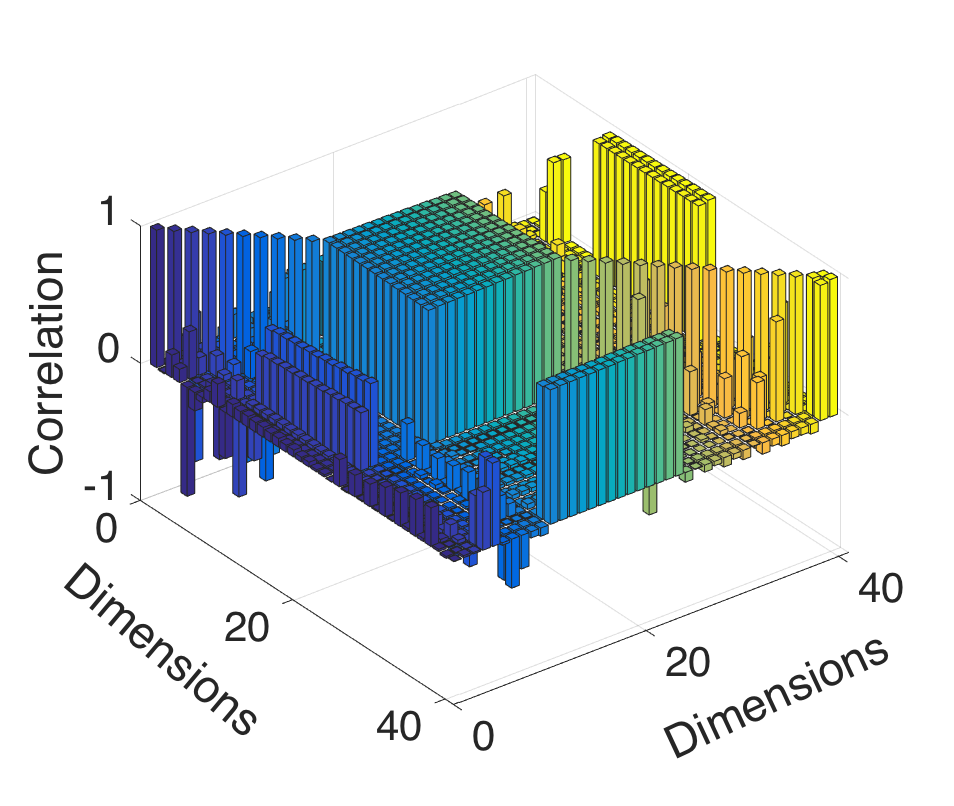
\includegraphics[width=0.9\textwidth]{figure/data2.eps}}
% \vspace{-0.1in}
\caption{A 40-dimensional dataset, Correlation between each dimension of \textbf{x}}
\label{fig:data2}
\end{minipage}
\vspace{-0.05in}
\end{figure}

\para{Dataset}
Given a such high-dimensional dataset, we decide to first analyze the relationship between each dimension.
As shown in Figure~\ref{fig:data2}, we can see that actually 16 dimensions of the 40-dimensional \textbf{x} are highly correlated to each other (correlation > 0.96).
So reducing the dimension of this dataset is a probable way to reduce the complexity of the algorithm.
Thus, we do this procedure by ignoring the \{12:24, 25:38\} dimensions, which are all highly correlated to the 11th dimension. And we consequently derive a 25-dimensional set.


%%% ABCD
\subsubsection{Auto Construction}
By conducting a greedy kernel search as in the previous experiment, we get a desired kernel function: \emph{SE}.

We hereby use this dataset to test the performance of different \emph{Likelihood Functions} and \emph{Inference Methods}.

\begin{table}[h]
\centering
{\small
\begin{tabular}{|c|cccc|}
    \hline
	    & exact & Laplace & VB & L00 \\ 
    \hline
	   Gaussian & & & & \\
	   Laplace & & & & \\
    \hline
\end{tabular}
}
\caption{MSE using different kinds of \emph{Likelihood Functions} and \emph{Inference Methods}. Different rows represents different \emph{Likelihood Functions} and different columns represents different \emph{Inference Methods}. }
\label{tab:predict21}
% \vspace{-0.05in}
\end{table}



%%% Additive Gaussian
\subsubsection{Additive Kernel}

%%%%
\para{Dataset Structure}
We surprisingly found that each dimension is gauss

%%%%
\para{Additive Kernel}
Since we have a 25-dimension(reduced) dataset, we set the kernel functions as:
\begin{equation}
\begin{aligned}
K_{add} &= \sum_{r=1}^{R} k_{add_{r}} (\textbf{x},\textbf{x}^{'}) \\
 &= \sum_{r=1}^{R} \{ \sigma^2_r \sum_{1 \leqslant i_1 < i_2 < ... < i_r \leqslant D} ( \prod_{d=1}^{r} k_{i_d} (\textbf{x}_{i_d},\textbf{x}_{i_d}^{'}) ) \}
\end{aligned}
\end{equation}
where 
\begin{equation}
k_{i_d} (\textbf{x}_{i_d},\textbf{x}_{i_d}^{'}) = SE = exp(-\frac{(\textbf{x}_{i_d}-\textbf{x}_{i_d}^{'})^{2}}{2l_{i_d}^{2}})
\end{equation}
We also use the same analysis method as in the last subsubsection, the result is shown in Table~\ref{tab:predict22}.

\begin{table}[h]
\centering
{\small
\begin{tabular}{|c|cccc|}
    \hline
	    & exact & Laplace & VB & L00 \\ 
    \hline
	   Gaussian & & & & \\
	   Laplace & & & & \\
    \hline
\end{tabular}
}
\caption{MSE using different kinds of \emph{Likelihood Functions} and \emph{Inference Methods}. Different rows represents different \emph{Likelihood Functions} and different columns represents different \emph{Inference Methods}. }
\label{tab:predict22}
% \vspace{-0.05in}
\end{table}









